\section{RiverSwim MDP [25 pts]}
Now you will implement value iteration and policy iteration for the RiverSwim environment (see picture below\footnote{Figure copied from \href{https://proceedings.neurips.cc/paper/2013/hash/6a5889bb0190d0211a991f47bb19a777-Abstract.html}{(Osband \& Van Roy, 2013)}.}) of \href{https://www.sciencedirect.com/science/article/pii/S0022000008000767}{(Strehl \& Littman, 2008)}.
\begin{figure}[h]
    \centering
    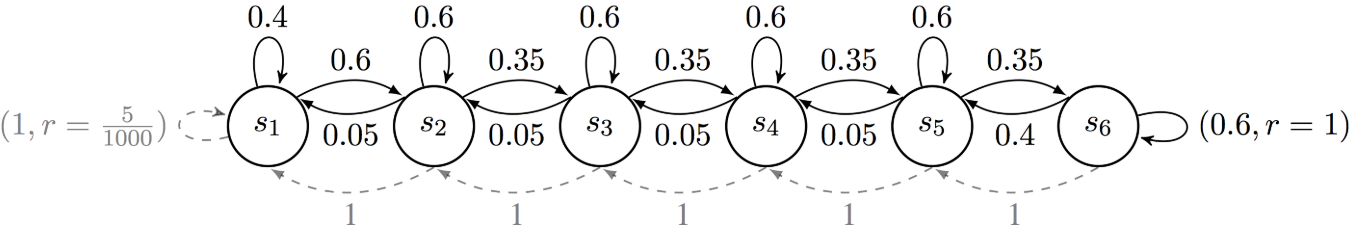
\includegraphics[width=\linewidth]{RiverSwim.png}
    \caption{The RiverSwim MDP where dashed and solid arrows represent transitions for the \textsc{LEFT} and \textsc{RIGHT} actions, respectively. The assignment uses a modified, customizable version of what is shown above where there are three different strengths (\textsc{WEAK}, \textsc{MEDIUM}, or \textsc{STRONG}) of the current (transition probabilities for being pushed back or successfully swimming \textsc{RIGHT}).}
    \label{fig:riverswim}
\end{figure}

\noindent \textbf{Setup:} This assignment needs to be completed with Python3 and \texttt{numpy}. 
% We have provided a \texttt{requirements.txt} file that contains all the associated Python libraries you will need to complete this assignment. You can go through the file and install all the libraries by running \texttt{pip install -r requirements.txt} in the terminal. We highly recommend that you do this in a \href{https://docs.python.org/3/library/venv.html}{virtual environment} dedicated for this assignment to avoid any dependency conflicts. 
% \textbf{While programming, please ignore any \texttt{DeprecationWarning} you may see}.
\\

\noindent \textbf{Submission:} There is a \texttt{Makefile} provided that will help you submit the assignment. Please run \texttt{make clean} followed by \texttt{make submit} in the terminal and submit the resulting zip file on Gradescope.


\begin{enumerate}[label=(\alph*)]
\item \textbf{(coding)} Read through \texttt{vi\_and\_pi.py} and implement \texttt{bellman\_backup}. Return the value associated with a single Bellman backup performed for an input state-action pair. [4 pts]\\


\item \textbf{(coding)} Implement \texttt{policy\_evaluation}, \texttt{policy\_improvement} and \texttt{policy\_iteration} in  \texttt{vi\_and\_pi.py}. Return the optimal value function and the optimal policy. [8pts]\\


\item \textbf{(coding)} Implement \texttt{value\_iteration} in \texttt{vi\_and\_pi.py}. Return the optimal value function and the optimal policy. [8 pts]\\


\item \textbf{(written)} Run both methods on RiverSwim with a \textsc{weak} current strength and find the largest discount factor (\textbf{only} up to two decimal places) such that an optimal agent starting in the initial far-left state (state $s_1$ in Figure \ref{fig:riverswim}) \textbf{does not} swim up the river (that is, does not go \textsc{RIGHT}). Using the value you find, interpret why this behavior makes sense. Now repeat this for RiverSwim with \textsc{medium} and \textsc{strong} currents, respectively. Describe and explain the changes in optimal values and discount factors you obtain both quantitatively and qualitatively. [5 pts]\\ \\
\textit{Sanity Check:} For RiverSwim with a discount factor $\gamma = 0.99$ and a \textsc{weak} current, the values for the left-most and right-most states ($s_1$ and $s_6$ in Figure \ref{fig:riverswim} above) are \texttt{30.328} and \texttt{36.859}. The value functions from VI and PI should be within error tolerance $10^{-3}$ of these values. You can use this to verify your implementation. For grading purposes, we shall test your implementation against other hidden test cases as well.

\end{enumerate}